\documentclass[11pt]{article}
\usepackage[margin=1in]{geometry}
\usepackage{lmodern}
\usepackage[T1]{fontenc}
\usepackage{amsmath,amssymb}
\usepackage{booktabs}
\usepackage{tabularx}
\usepackage{enumitem}
\usepackage{xcolor}
\usepackage{float}
\usepackage{tikz}
\usetikzlibrary{positioning,fit,arrows.meta,shapes.geometric,calc}
\usepackage{hyperref}
\hypersetup{colorlinks=true,linkcolor=blue!50!black,urlcolor=blue!50!black}

\setlist{itemsep=2pt,topsep=4pt}
\setlength{\emergencystretch}{3em}
\newcommand{\code}[1]{\texttt{#1}}
\newcolumntype{L}{>{\raggedright\arraybackslash}X}
\definecolor{svc}{RGB}{226,236,250}
\definecolor{agt}{RGB}{232,245,233}
\definecolor{ext}{RGB}{250,240,225}
\definecolor{hum}{RGB}{245,232,245}

\title{\textbf{Agentic Lab}\\[4pt]\large Architecture: roles, logic, conventions}
\author{Framework reference, as of the merge of PR \#13}
\date{October 2026}

\begin{document}
\maketitle

\begin{abstract}
Agentic Lab is a framework in which a small team of humans and AI agents run a scientific
lab together. Members talk to their \emph{manager} agents in Slack; managers delegate work
to \emph{worker} agents on GPU machines; a \emph{secretary} keeps the lab running. Every
agent runs Claude (through the Claude Agent SDK) on a human member's Claude seat, inside
Claude Code's built-in sandbox, as its own Unix user. Anything an agent can't do inside its
sandbox is asked of a human in a Slack DM. The lab is described by one file,
\code{lab.yaml}, kept in the lab's private configuration repository; only what is merged
to that repository's \code{main} is ever deployed. This document describes the roles, the
mechanisms that bind them together, and the conventions the framework relies on.
\end{abstract}

\tableofcontents
\newpage

%=====================================================================
\section{Principles}

\begin{enumerate}
  \item \textbf{Humans decide, agents do.} Agents never approve anything: not each other's
    actions, not their own, not pull requests. Approvals come from the human the action is
    for, in a Slack DM, from a dedicated app.
  \item \textbf{Sandbox the environment, not the commands.} There is no command parsing or
    classifier. Inside Claude Code's sandbox an agent may do anything; leaving it (the
    internet, writes outside its folders) needs a human.
  \item \textbf{Secrets belong to services, not to agents.} Each agent's service holds its
    tokens in a folder the agent's sandbox can't read. Secrets never pass through a chat:
    they arrive through one-time links and hidden prompts.
  \item \textbf{One file describes the lab, and git is its history.} \code{lab.yaml}
    declares humans, agents, hosts and grants. Every change is a reviewed pull request in
    the lab's private configuration repository; deployment takes only \code{main}.
  \item \textbf{Every agent is attached to a human, in terms of tokens.} An agent runs on
    one member's Claude seat. Who may \emph{use} an agent is a separate setting.
  \item \textbf{Transparency over limits.} No spend limits; instead the web UI and the
    secretary show usage per Claude account, with when and from where each number was read.
  \item \textbf{Simple, generic, portable.} No hard-coded hosts, organisations or project
    tools. Experiment trackers and similar tools are extensions a lab adds itself.
\end{enumerate}

%=====================================================================
\section{Roles}

\subsection{Humans}
\begin{description}
  \item[Member] A person in \code{lab.yaml} (\code{humans:}), with a Slack member id. Talks
    to managers and the secretary in Slack, receives the approvals for work done for them,
    and lends their Claude seat to the agents attached to them.
  \item[Admin] A member with \code{admin: true} and a \code{tailscale\_login}. Only admins
    can read agents' logs in the web UI, change the lab (through the secretary or the
    console), deploy, power off a busy machine, or ask for someone else's token.
\end{description}

\subsection{Agents}
\begin{description}
  \item[Secretary] Exactly one per lab, on an always-on host. Keeps the lab running: collects
    its state, serves the web UI, powers cloud machines on and off (and stops idle ones),
    warns about expiring tokens, answers questions about the lab in Slack, and is how
    admins administer the lab after the install (\S\ref{sec:selfadmin}). It refuses research
    work and points to the member's manager.
  \item[Manager] A member's team-mate in Slack: it understands requests, delegates work to
    workers, follows the tasks and reports back with summaries, plots and files. It never
    approves; it relays. A manager is \emph{dedicated} (serves one member) or \emph{shared}
    (serves every member, with a separate memory for each).
  \item[Worker] An agent on a GPU machine that takes tasks over MCP, one at a time, first
    come first served, and reports progress and a result. Also \emph{dedicated} or
    \emph{shared}.
\end{description}

\subsection{Services that are not agents}
\begin{description}
  \item[Broker] On the secretary host, as \code{lab-broker}. Receives every permission
    request from every agent, works out which human decides, and asks them through the
    \emph{Lab Approvals} Slack app. Holds active grants.
  \item[Intake] On the secretary host. Receives secrets through one-time codes: web forms
    (\code{/s/<code>}) and a small client script for Claude tokens.
\end{description}

\subsection{Hosts}
\begin{itemize}
  \item \textbf{Secretary host}: small, always on (on-prem or a small VM). Runs the
    secretary, broker, intake and web UI, and the admin's Claude Code session for the
    install.
  \item \textbf{Managers} run on any host: the secretary host, a CPU VM of their own, or a
    GPU VM next to the workers they use. Each manager's \code{host:} in \code{lab.yaml}
    says where; several agents on one host still each have their own Unix user.
  \item \textbf{GPU hosts}: cloud VMs (Nebius in this version), \code{power: on\_demand} or
    \code{always\_on}, stopped when idle.
  \item All hosts are on one \textbf{Tailscale tailnet}; services talk to each other only
    over it.
\end{itemize}

%=====================================================================
\section{The big picture}

\begin{figure}[H]
\centering
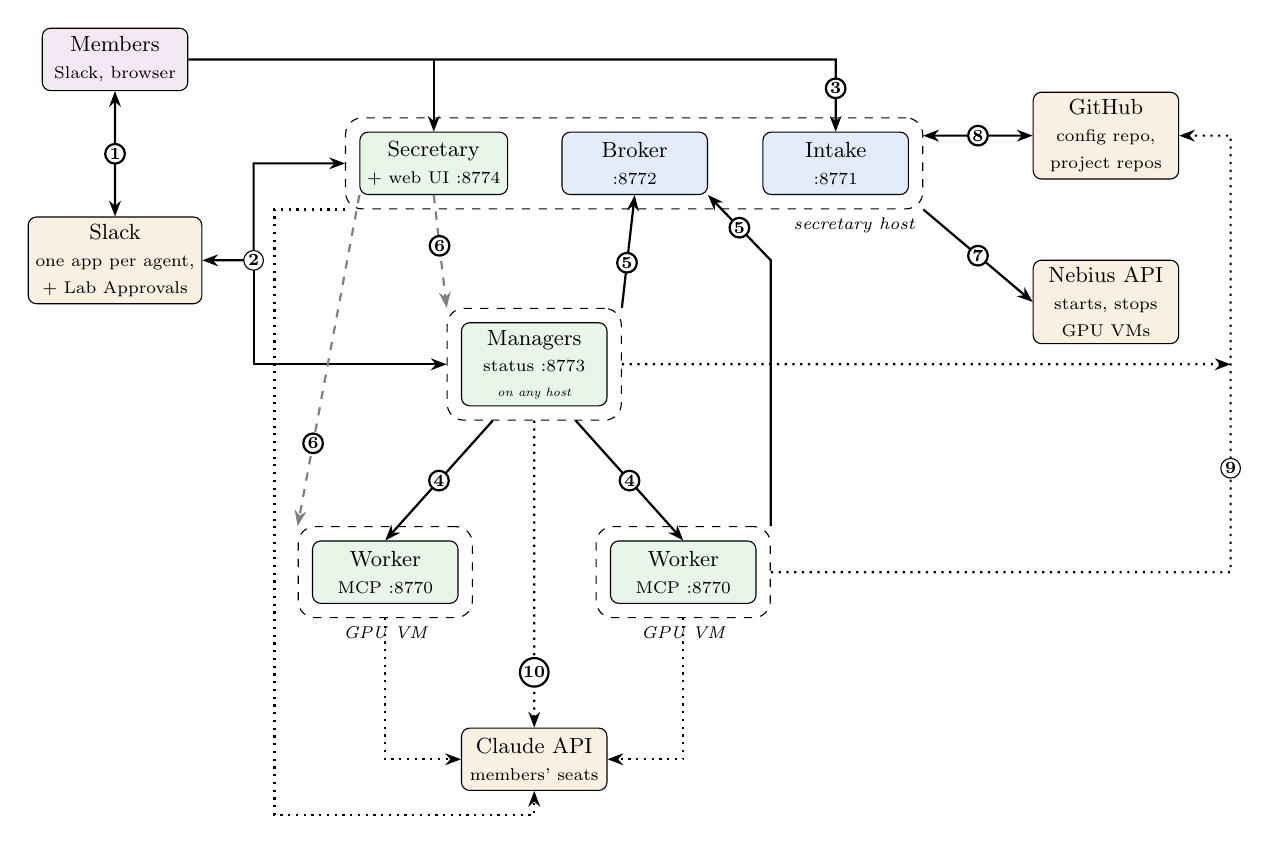
\begin{tikzpicture}[scale=0.88, transform shape,
  box/.style={draw, rounded corners=3pt, align=center, font=\small, inner sep=3pt,
              minimum height=9mm, minimum width=21mm},
  host/.style={draw, dashed, rounded corners=6pt, inner sep=5pt},
  hl/.style={font=\scriptsize\itshape},
  n/.style={circle, draw=black, solid, fill=white, text=black, inner sep=0.6pt,
            font=\scriptsize\bfseries},
  ar/.style={-{Stealth[length=2mm]}, thick},
  da/.style={{Stealth[length=2mm]}-{Stealth[length=2mm]}, thick},
  mon/.style={-{Stealth[length=2mm]}, thick, gray, dashed},
  dt/.style={-{Stealth[length=2mm]}, thick, dotted}
]
% ---- secretary host
\node[box, fill=agt] (sec) at (0,2) {Secretary\\\scriptsize + web UI :8774};
\node[box, fill=svc] (bro) at (2.9,2) {Broker\\\scriptsize :8772};
\node[box, fill=svc] (int) at (5.8,2) {Intake\\\scriptsize :8771};
\node[host, fit=(sec)(bro)(int), label={[hl, anchor=north east]south east:secretary host}] (sh) {};
% ---- managers (on their own host, or on the secretary host)
\node[box, fill=agt] (mgr) at (1.45,-0.9) {Managers\\\scriptsize status :8773\\[-1pt]
      \tiny\itshape on any host};
\node[host, fit=(mgr)] (mh) {};
% ---- GPU VMs
\node[box, fill=agt] (w1) at (-0.7,-3.9) {Worker\\\scriptsize MCP :8770};
\node[host, fit=(w1), label={[hl]below:GPU VM}] (g1) {};
\node[box, fill=agt] (w2) at (3.6,-3.9) {Worker\\\scriptsize MCP :8770};
\node[host, fit=(w2), label={[hl]below:GPU VM}] (g2) {};
% ---- people and outside services
\node[box, fill=hum] (hum) at (-4.6,3.5) {Members\\\scriptsize Slack, browser};
\node[box, fill=ext] (slack) at (-4.6,0.6) {Slack\\\scriptsize one app per agent,\\\scriptsize + Lab Approvals};
\node[box, fill=ext] (gh) at (9.7,2.4) {GitHub\\\scriptsize config repo,\\\scriptsize project repos};
\node[box, fill=ext] (neb) at (9.7,0.0) {Nebius API\\\scriptsize starts, stops\\\scriptsize GPU VMs};
\node[box, fill=ext] (cl) at (1.45,-6.6) {Claude API\\\scriptsize members' seats};
% ---- 1 members <-> Slack
\draw[da] (hum) -- node[n]{1} (slack);
% ---- 2 Slack <-> the apps (they connect out: Socket Mode)
\draw[da] (slack.east) -- (-2.6,0.6) |- (sh.west);
\draw[ar] (-2.6,0.6) |- (mh.west);
\node[n] at (-2.6,0.6) {2};
% ---- 3 members' browsers and laptops: web UI, intake
\draw[ar] (hum.east) -- (5.8,3.5) -- node[n, pos=0.4]{3} (int.north);
\draw[ar] (0,3.5) -- (sec.north);
% ---- 4 tasks and files
\draw[ar] (mh.south) ++(-0.6,0) -- node[n]{4} (w1.north);
\draw[ar] (mh.south) ++(0.6,0) -- node[n]{4} (w2.north);
% ---- 5 permission requests to the broker
\draw[ar] (mh.north east) -- node[n, pos=0.4]{5} (bro.south);
\draw[ar] (g2.north east) -- (g2.north east |- 0,0.6) -- node[n, pos=0.5]{5} (bro.south east);
% ---- 6 monitoring (read-only) and deploys (SSH)
\draw[mon] (sec.south) -- node[n, pos=0.45]{6} (mh.north west);
\draw[mon] (sec.south west) -- node[n, pos=0.75]{6} (g1.north west);
% ---- 7 VM power, 8 config repo
\draw[ar] (sh.south east) -- node[n]{7} (neb.west);
\draw[da] (sh.east |- gh) -- node[n]{8} (gh);
% ---- 9 bots on project repos
\draw[dt] (g2.east) -- (11.5,-3.9) |- (gh.east);
\draw[dt] (mh.east) -- (11.5,-0.9);
\node[n] at (11.5,-2.4) {9};
% ---- 10 every agent calls Claude
\draw[dt] (g1.south) |- (cl.west);
\draw[dt] (g2.south) |- (cl.east);
\draw[dt] (mh.south) -- node[n, pos=0.82]{10} (cl.north);
\draw[dt] (sh.south west) -| (-2.3,-7.4) -| (cl.south);
\end{tikzpicture}


\caption{Components and connections. Dashed boxes are hosts; all traffic between lab hosts
runs over the tailnet. Slack, GitHub, Nebius and Claude are reached over the internet by the
services, never by sandboxed agent commands, except GitHub for an agent with a bot (9).}
\end{figure}

\noindent\textbf{The numbered connections in Figure~1:}\par
\small
\begin{tabularx}{\linewidth}{rL}
1 & Members talk to agents and answer approvals in Slack (DMs, threads, buttons). \\
2 & Each Slack-facing agent has its own Slack app (the secretary, every manager), the broker
    has \emph{Lab Approvals}; all connect \emph{out} to Slack (Socket Mode, no public URL). \\
3 & Over the tailnet: members' browsers open the web UI (served by the secretary); their
    laptops hand secrets to the intake (one-time links and codes). \\
4 & Managers give workers tasks and exchange files with them (MCP, a token per pair). \\
5 & Every worker and every manager sends its permission requests to the broker, which asks
    the human the action is for (2, 1). \\
6 & The secretary monitors workers (MCP, read-only token), managers (status endpoint) and the
    broker; \code{lab apply}/\code{apply-main} deploy from this host to every host over SSH. \\
7 & The secretary starts and stops the GPU VMs through the Nebius API. \\
8 & Deploys fetch the config repo's \code{main}; the secretary pushes branches for review. \\
9 & Managers and workers with a GitHub bot reach github.com from their sandboxes. \\
10 & Every agent (the secretary too) runs Claude on its member's seat. \\
\end{tabularx}
\normalsize


A typical piece of work:
\begin{enumerate}
  \item A member DMs their manager: \emph{``train the baseline on worker-a and show me the
    loss curve''}.
  \item The manager submits a task to the worker over MCP, naming the member as the
    requester, and registers it with the broker.
  \item The worker runs the task in its sandbox, reporting progress. If it needs something
    outside the sandbox (say, a dataset from the internet) it asks; the broker DMs
    \emph{the requester} with buttons; the answer comes back to the worker.
  \item The manager follows the task and posts progress, the plot and a summary in the
    member's thread. The secretary's web UI shows it all as it happens.
\end{enumerate}

%=====================================================================
\section{Identity, users and tokens}

\begin{itemize}
  \item \textbf{One Unix user per agent}: \code{lab-<agent id>} (a system user, no login
    shell, no SSH keys, home folder mode 700). Several agents on one host never share a
    user, so they can't read each other's files. Humans log in as themselves.
  \item Each agent runs as a \textbf{systemd service} under its user:
    \code{lab-worker@<id>}, \code{lab-manager@<id>}, \code{lab-secretary}; plus
    \code{lab-broker} and \code{lab-intake}.
  \item \textbf{Folders per agent user}:
    \begin{itemize}
      \item \code{\textasciitilde/work}: its working folder (writable in its sandbox);
      \item \code{\textasciitilde/.config/agentic-lab}: its service's secrets (Claude token,
        Slack tokens, lab tokens, GitHub token), \emph{not readable} by its sandbox;
      \item \code{\textasciitilde/.local/state/agentic-lab}: the service's state (task
        queue, memory, usage, event log), \emph{not readable} by its sandbox.
    \end{itemize}
  \item \textbf{Claude}: \code{human:} on an agent says whose Claude seat it runs on (a
    \code{claude setup-token} token, valid a year). The token reaches Claude Code as an
    environment variable that is stripped from sandboxed commands.
  \item \textbf{Lab tokens}: generated by \code{lab apply} and never shown; each pair of
    services that talk has its own (manager$\to$worker, agent$\to$broker, the secretary's
    \emph{read-only} monitoring tokens). They live in
    \code{/etc/agentic-lab/private/tokens.yaml} (root) and in the services' secret folders.
  \item \textbf{Display names}: every agent has an id (\code{mgr-flash}) and a
    \code{display\_name} (\emph{Flash}), the name humans see. Names are the admin's choice;
    the framework and its guide never invent them.
\end{itemize}

%=====================================================================
\section{The sandbox and permissions}

\subsection{Inside the sandbox: no questions}
Every agent's Claude Code runs with the built-in sandbox (bubblewrap + seccomp), rendered
per agent from \code{lab.yaml} (\code{lab settings <agent>} prints it):
\begin{itemize}
  \item \textbf{Network}: only the lab's tailnet names (\code{*.<tailnet>}), plus hosts
    granted to it; strict allowlist (unknown hosts are refused, not prompted). Raw IPs are
    refused: lab resources are reached by their tailnet names.
  \item \textbf{Files}: writes only in the working folder, \code{/tmp} and granted paths;
    reads anywhere except \code{/run}, \code{/var/run} and its service's secret and
    state folders.
  \item \textbf{GPU}: workers see the GPU through a wrapper around bubblewrap
    (\code{bwrap-gpu}, set as \code{sandbox.bwrapPath} in Claude Code's managed settings)
    that binds the NVIDIA devices; Unix sockets are allowed for CUDA, and \code{/run} is
    hidden instead (closing a \code{systemd-run} escape).
  \item \textbf{Host setup} (\code{setup-sandbox.sh}): an AppArmor profile that lets
    bubblewrap create its namespaces on Ubuntu, the GPU wrapper, the managed settings.
\end{itemize}
Any Bash command that stays in the sandbox is allowed without asking. Caches
(\code{XDG\_CACHE\_HOME}) point into the working folder. Managers auto-compact their context
at 17\% of the window (\code{compact\_percent}); others at Claude's default.

\subsection{Outside the sandbox: a human decides}
When the sandbox refuses something, the agent sees why and may retry outside it. That
retry is a permission request: the agent's service sends it to the broker, with the
sandbox violations that explain it.

\begin{description}
  \item[Who decides] The human \emph{the action is for}: a worker task's requester (as
    registered by the manager that submitted it, not as claimed by the worker); for a
    manager, the member whose message started the work. Never an agent.
  \item[How] A DM from the \emph{Lab Approvals} app with buttons: \textbf{Run once},
    \textbf{Allow \emph{X} for 1 hour}, \textbf{Allow \emph{X} for this task}, \textbf{Deny}.
    A reply in the DM's thread denies, with the reply as the reason.
  \item[Timeout] Unanswered requests are denied (default 120 s per human,
    \code{timeout\_s}); a timeout never approves.
  \item[Grants] ``For a while'' answers become \emph{grants} that widen the sandbox
    (a domain, a writable path, or a tool) with an expiry; the agent's session restarts
    with the wider sandbox. \emph{Standing} grants are written in \code{lab.yaml}.
    ``Trust everything unsandboxed for an hour'' does not exist.
  \item[Managers] relay: they can show members what their tasks are waiting for and add
    context to a pending request; they cannot decide it.
\end{description}

%=====================================================================
\section{Work: managers and workers}

\subsection{Workers}
\begin{itemize}
  \item An MCP server on the tailnet (\code{http://<host>:8770/mcp}), authenticated by
    bearer tokens: one per manager allowed to use it, plus the secretary's read-only one.
  \item Its tools:\\ \code{submit\_task}, \code{task\_status}, \code{task\_result},
    \code{cancel\_task}, \code{list\_tasks}, \code{get\_guardrails}, \code{read\_file}
    and \code{write\_file} (its working folder, up to 20 MB), \code{health\_check}
    (queue, GPU and its processes, disk, usage), \code{check\_usage}, and
    \code{recent\_events} (its log: \emph{the secretary's token only}).
  \item Tasks run one at a time, first come first served; a restart requeues a running
    task and resumes its Claude session. No fixed results contract: a result is a summary
    plus whatever artifacts fit (files, commits, links).
\end{itemize}

\subsection{Managers}
\begin{itemize}
  \item \textbf{Slack}: Socket Mode (no public URL). A DM is one conversation; in channels a
    manager joins only threads where it's mentioned or already involved, reading the thread
    so far (up to 50 messages) on first mention. In such a thread it sees every message and
    may stay silent. Attachments (up to 50 MB) are downloaded into its working folder.
  \item Every message is checked against \code{lab.yaml}: only lab members, and only those
    who may use this manager.
  \item \textbf{Tools}: list workers, submit and follow tasks, pending approvals and notes
    on them, post files, fetch a worker's file into the conversation, send a file to a
    worker, \code{recall} and \code{remember}.
  \item \textbf{Memory}: durable notes about members and their work. A dedicated manager has
    one memory; a shared manager keeps one per member, separated by code (private
    conversations stay private).
  \item \textbf{Follow-up}: a background loop posts each task's progress and result in the
    conversation that started it, mentioning the requester.
  \item \textbf{Staying reachable}: a manager runs one turn at a time \emph{per
    conversation} (other threads and members are never blocked). It does work itself only
    when it takes a few minutes (an issue, a comment, a small fix); longer work and
    anything needing a GPU goes to a worker. A turn longer than \code{turn\_budget\_min}
    (default 5) is interrupted, and the manager gets one short turn (90 s) to say where it
    got to or hand the rest to a worker. A message arriving while it's busy in that
    conversation gets an immediate ``still working on the previous message'' reply.
\end{itemize}

\subsection{Who may use what}
\begin{tabularx}{\linewidth}{lL}
\toprule
\code{access} & Meaning \\
\midrule
\code{dedicated} & Only the agent's own member (\code{human:}) may use it; a dedicated worker
  takes tasks only from its member's managers. \\
\code{shared} & Every member may use it; a shared manager keeps per-member memory. \\
\bottomrule
\end{tabularx}

%=====================================================================
\section{The secretary}

\subsection{State and the web UI}
Every 15 s the secretary collects the lab's state: workers (over MCP, with its read-only
token), managers (their status endpoint), the broker (pending approvals, grants), local
services (systemd) and machines (Nebius, every few rounds). It serves:
\begin{itemize}
  \item \textbf{The web UI} (\code{http://<secretary host>:8774/}, tailnet only, refreshes
    every 20 s): Claude usage per account, workers and their tasks, approvals and grants,
    machines, agents, and which configuration and framework commits are deployed.
  \item \textbf{Agents' logs} (\code{/logs/<agent>}), \textbf{admins only}: the request's
    tailnet address must not be a lab host; \code{tailscale whois} must name a person (not
    a tagged device) whose login is an admin's in \code{lab.yaml}. Tailscale authenticates
    every packet with the device's key, so the address can't be forged.
  \item \textbf{A Slack Home tab}: a personal digest (your usage, your tasks, approvals
    waiting for you, machines) with a link to the web UI.
\end{itemize}

\subsection{Claude usage}
\begin{itemize}
  \item Each agent records its tokens per run (new vs.\ cached) and its seat's limit
    readings. Readings are per account (a seat is shared by all its agents); the freshest
    wins, and every number shows \emph{as of when} and \emph{from which agent}.
  \item Percentages come from a \textbf{probe}: every API reply carries the seat's 5-hour
    and weekly utilization in headers, which Claude Code doesn't pass on. Each agent's
    service sends one tiny request (Haiku, 1 output token) every 10 minutes, only while
    its seat's 5-hour window is known to be open, so it never opens one.
  \item \textbf{Check now} on each account in the web UI asks one agent on that seat to
    probe at once (once a minute at most).
\end{itemize}

\subsection{Machines}
\begin{itemize}
  \item \textbf{Power}: the secretary starts and stops Nebius VMs listed in \code{lab.yaml}
    (\code{kind: cloud}, \code{provider: nebius}, \code{instance}), with a service account
    that may only view, start and stop VMs. Never its own host.
  \item \textbf{Busy} means: a worker there has a task running, queued or awaiting
    approval; or any process on a GPU (anyone's, not only the lab's); or a GPU at 10\% or
    more; or a manager runs there.
  \item \textbf{Idle stop}: an \code{on\_demand} host with only workers is stopped after
    \code{idle\_stop\_min} minutes of not being busy.
  \item \textbf{Who may power}: any member may power a machine on, or off when idle;
    powering off a busy machine is for admins only, after confirming (\code{force\_off}).
\end{itemize}

\subsection{Notices}
Daily, the secretary warns about credentials and GitHub bot tokens expiring within 14 days
(from \code{lab.yaml}) and can post lab-wide notices to an \code{announcements} channel.

%=====================================================================
\section{Configuration: lab.yaml and the config repository}

\subsection{lab.yaml}
\begin{tabularx}{\linewidth}{lL}
\toprule
Section & Contents \\
\midrule
\code{lab}, \code{tailnet} & The lab's name; the tailnet's DNS suffix. \\
\code{humans} & Members: \code{name}, \code{slack\_user}, \code{channels} (permissions:
  Slack DM), \code{admin}, \code{tailscale\_login}. \\
\code{agents} & Each agent: \code{role}, \code{human} (whose seat), \code{host},
  \code{access}, \code{display\_name}, \code{grants} (standing), \code{github} (its bot),
  \code{model}, \code{workdir}, \code{port}, \code{compact\_percent}, \code{slack\_app},
  \code{turn\_budget\_min} (managers). \\
\code{hosts} & \code{kind} (onprem/cloud), \code{provider}, \code{instance},
  \code{power}, \code{idle\_stop\_min}, \code{tailnet\_name}, \code{ssh\_user}. \\
\code{github} & \code{accounts}: the bots, with their commit \code{email} and token
  \code{expires}. \\
\code{credentials} & Other expiring credentials to be reminded of. \\
\code{announcements} & A Slack channel for lab-wide notices. \\
\bottomrule
\end{tabularx}

\medskip
\code{lab check} validates everything at once (unknown keys are errors) and warns about what
is merely odd. Agent ids are lowercase (\code{[a-z][a-z0-9-]*}), since they become Unix
user names.

\subsection{Only reviewed configuration is deployed}
\begin{itemize}
  \item The lab's configuration lives in its own \textbf{private repository}:
    \code{lab.yaml} and \code{framework.lock}, which pins the framework to one commit. The
    framework repository is only read.
  \item \code{lab apply} fetches the config repository and deploys \code{lab.yaml} and
    \code{framework.lock} \emph{as they are on} \code{origin/main}, never the working copy.
    It ships the framework only from a clean checkout at the pinned commit.
  \item Every change: a branch $\to$ \code{lab plan --working-tree} (preview) $\to$ a pull
    request (\code{lab pr-link}) $\to$ a human reviews and merges $\to$ \code{lab apply}.
    Upgrading the framework is the same: \code{--update-framework} only rewrites
    \code{framework.lock}; the new pin goes through a pull request.
  \item Every host records what it runs in \code{/etc/agentic-lab/applied.yaml} (config and
    framework commits, when, by whom), shown by \code{lab doctor} and the web UI.
  \item \textbf{Break glass}: \code{lab apply --unreviewed} deploys the working copy; every
    host flags it as unreviewed until a reviewed deploy replaces it.
\end{itemize}

\subsection{What lab apply does}
From the secretary host, as root, for each host (locally, or over SSH as the admin with
passwordless sudo): ship the framework to \code{/opt/agentic-lab} (and \code{lab} on the
PATH), install \code{lab.yaml}, set up the sandbox, create the agents' users, install their
secrets and generated tokens, install and (re)start their services. Services whose secrets
haven't arrived yet are installed but held. Every step is idempotent: re-running is safe.
\code{lab doctor} checks a host against \code{lab.yaml} and says how to fix each failure.

%=====================================================================
\section{Administering the lab from Slack}\label{sec:selfadmin}

After the install, admins work with the secretary in a DM; the console is for the install
and emergencies. Admin-only tools, checked in code (the person's Slack identity must be an
admin's in \code{lab.yaml}):
\begin{description}
  \item[\code{propose\_lab\_change}] writes the whole new \code{lab.yaml} on a branch of the
    secretary's own clone of the config repository, checks it, pushes it, and replies with
    the diff and the pull request link: \emph{``here is the PR, review and merge it''}. It
    never touches \code{main}.
  \item[\code{offer\_deploy}] after the merge, posts a \textbf{Deploy} button listing what
    is merged but not deployed. Only an admin's click deploys; a button left behind by a
    newer \code{main} refuses. The result is posted back in the conversation.
  \item[\code{request\_slack\_app}, \code{request\_github\_token}] post the steps (manifest,
    links, clicks) and a one-time link for a new manager's Slack app or a bot's token.
  \item[\code{check\_slack\_app}, \code{read\_lab\_config}] check a Slack app's tokens; read
    the configuration on \code{main}.
\end{description}

\textbf{The secretary's one root command} is \code{lab apply-main}, allowed by a sudoers
rule with no arguments: it deploys only the config repository's \code{main}, moving the
framework checkout to the pinned commit, as its own systemd unit (so it survives the
secretary's own restart). Even a misled secretary can only deploy what a human merged.
Its deploy key (write: it pushes branches, never merges) and its clone live in folders its
sandbox can't read.

\textbf{Still at the console}: the install itself; creating the first Slack apps; giving a
new GPU VM SSH access; removing an agent's Unix user; \code{--unreviewed}; uninstalling
(\code{docs/uninstall.md}).

%=====================================================================
\section{Secrets}

\begin{tabularx}{\linewidth}{lL}
\toprule
Secret & How it arrives \\
\midrule
A member's Claude token & The secretary DMs them a one-time command. On their own computer
  it runs \code{claude setup-token} and sends the token straight to the intake over the
  tailnet; the intake checks it with Anthropic. Fallback: a hidden prompt. \\
A Slack app's tokens & A one-time web form (bot token \code{xoxb-}, app token
  \code{xapp-}); \code{lab slack-verify} checks them with Slack. \\
A GitHub bot's token & A one-time web form; the intake checks with GitHub that it is that
  bot's. \\
Nebius service account & \code{lab nebius connect} (key generated on the host), or a form. \\
Lab tokens & Generated by \code{lab apply}; never shown. \\
\bottomrule
\end{tabularx}

\medskip
One-time codes expire after 24 h and are used once; failed attempts are rate-limited.
Rules: no secret in any chat (Slack or Claude); agents can't read their service's secrets;
an agent asked to recite a token refuses.

%=====================================================================
\section{GitHub for agents}\label{sec:github}

\begin{itemize}
  \item A manager or worker may have \textbf{one GitHub identity}: a bot account (a GitHub
    machine user) named in \code{lab.yaml} (\code{github: <bot>} on the agent, the bot in
    \code{github.accounts}). Several agents may share one bot.
  \item The bot's token is in the agent's environment (\code{GH\_TOKEN}) for all its work;
    git authenticates through a credential helper and commits carry the bot's name and
    email; \code{gh} is installed; \code{github.com} is reachable from its sandbox.
  \item The agent \emph{can} read that token. What keeps this safe is GitHub: private
    repositories, a fine-grained token limited to the lab's repositories (contents, pull
    requests, issues), and \textbf{branch protection} on \code{main} (pull requests only,
    reviews by human code owners, no bypass for bots). Bots push branches and open pull
    requests, issues and comments; their approval never counts and they can't merge.
\end{itemize}

%=====================================================================
\section{Observability}
\begin{itemize}
  \item \textbf{Event logs}: each agent's service writes its own log (messages, replies,
    tool calls, approvals, task events), one JSON-lines file per day, kept 14 days, in its
    state folder. The agent can't read it.
  \item \textbf{Reading logs}: the web UI (admins), \code{sudo lab logs <agent>} on its
    host. Workers hand their log only to the secretary's monitoring token; managers'
    status endpoint likewise.
  \item \textbf{Debugging}: \code{sudo lab debug <agent>} stops its service and opens its
    latest session in the classic Claude Code console, as its user with its sandbox;
    \code{lab manager ask} and \code{lab secretary ask} talk to them without Slack.
\end{itemize}

%=====================================================================
\section{Security summary}

\begin{tabularx}{\linewidth}{lL}
\toprule
Boundary & What enforces it \\
\midrule
Agent vs.\ the internet and the host & Claude Code's sandbox (strict network allowlist,
  write allowlist, hidden secrets and \code{/run}); leaving it needs a human. \\
Agent vs.\ agent & One Unix user per agent; lab tokens per pair of services; a worker
  accepts only its allowed managers. \\
Who approves & The broker asks the human the action is for; timeouts deny; agents have no
  way to approve. \\
Who changes the lab & Merged pull requests on the config repository; \code{lab apply} and
  \code{apply-main} deploy only \code{main}; Slack admin tools check the admin in code. \\
Who reads logs & Tailscale identity matched to \code{admin: true}; lab hosts and tagged
  devices refused. \\
Secrets & Services' folders unreadable by sandboxes; one-time intake; no chat. \\
GitHub & Private repos, fine-grained tokens, branch protection. \\
\bottomrule
\end{tabularx}

\medskip
\textbf{Residual risks, by design}: anyone with \code{sudo} on a lab host is effectively an
admin there; an admin's device and Tailscale login are the keys to the logs; the web UI's
main page is visible to the whole tailnet (restrict it with Tailscale ACLs); a GitHub bot's
token is readable by its agents.

%=====================================================================
\section{Conventions}
\begin{itemize}
  \item \textbf{Names}: agents' display names are chosen by the admin, never invented; ids
    derive from them (\code{Flash} $\to$ \code{mgr-flash}); Unix users are
    \code{lab-<id>}; services \code{lab-<role>@<id>}.
  \item \textbf{Ports} (tailnet only): worker MCP 8770, intake 8771, broker 8772, manager
    status 8773, secretary web UI 8774.
  \item \textbf{Paths}:
    \begin{itemize}
      \item framework: \code{/opt/agentic-lab}; deploy logs: \code{/var/log/agentic-lab};
      \item configuration: \code{/etc/agentic-lab} (\code{lab.yaml},
        \code{applied.yaml}, \code{private/});
      \item per agent: \code{\textasciitilde/work}, \code{\textasciitilde/.config/agentic-lab}
        (secrets), \code{\textasciitilde/.local/state/agentic-lab} (state).
    \end{itemize}
  \item \textbf{Changes}: branch $\to$ pull request $\to$ human merge $\to$ deploy, for the
    lab's configuration and the framework alike.
  \item \textbf{Slack apps}: one per Slack-facing agent (each manager, the secretary) and
    one \emph{Lab Approvals} app for the broker; manifests generated by
    \code{lab slack-manifest}; created one at a time, verified before the next.
  \item \textbf{Guidance}: the admin's own Claude Code session follows the repository's
    \code{lab-admin} skill and \code{docs/install.md}: explain before acting, ask rather than
    assume (names, ids), derive rather than ask (App IDs, tailnet names), never take a
    secret in the chat.
\end{itemize}

%=====================================================================
\section{Command reference}
\begin{tabularx}{\linewidth}{lL}
\toprule
Command & Purpose \\
\midrule
\code{lab init} & Write the first \code{lab.yaml} (and \code{framework.lock}). \\
\code{lab check} & Validate \code{lab.yaml}. \\
\code{lab plan [--working-tree]} & What a deploy would do; missing secrets. \\
\code{lab apply [--update-framework] [--unreviewed]} & Deploy \code{main} (sudo). \\
\code{lab apply-main} & The secretary's deploy of \code{main} (sudoers). \\
\code{lab pr-link} & The link to open a pull request for the config branch. \\
\code{lab doctor} & Check this host; every failure says how to fix it. \\
\code{lab secret request} & A one-time code or link for a secret. \\
\code{lab slack-manifest}, \code{lab slack-verify} & A Slack app's manifest; check its tokens. \\
\code{lab nebius connect} & Set up VM power with one admin login. \\
\code{lab settings <agent>} & The agent's rendered sandbox settings. \\
\code{lab logs}, \code{lab debug} & An agent's log; its session in the console. \\
\code{lab manager ask}, \code{lab secretary ask} & Talk to them without Slack. \\
\bottomrule
\end{tabularx}

%=====================================================================
\section{Not in this version}
\begin{itemize}
  \item Per-token (API) billing: agents run on members' Claude seats only.
  \item Permission channels other than Slack DM; approvals in the web UI (it monitors only).
  \item Several GitHub identities per agent, or switching identity per task.
  \item Cloud providers other than Nebius for VM power.
  \item An uninstall command (\code{docs/uninstall.md} describes the steps).
  \item Project tools such as experiment trackers: extensions a lab builds itself.
\end{itemize}

\end{document}
